%----------------------------------------------------------------------------------------
\section{Design of the WSN Test-Bed}


%------------------------------------------------------------------
\subsection{Presentation of the thesis goal}
The purpose of this thesis is creating a wireless sensor network in the GroupT Vesalius building. It is not our goal to cover the entire building with sensors but rather establish a basic wireless sensor network which reaches out throughout the entire building. So that later on sensor nodes can be added and they will be easy to integrate with the existing network. The data coming from these sensors should also be stored safely and a web interface should allow easy access to all data. For data storage Ipsum is used, this is a cloud storage system developed by Ruben Taqc. Ipsum is already used to log data coming from other sensors and is still being updated and maintained. The web interface is a master thesis of Matthias Verhelst. For normal users the web interface should fetch data from Ipsum. But for admin or privileged users it should also possible to communicate directly with the wireless sensor network. So the gateway has to have a web service running that can be contacted by clients via a web browser. Since wireless sensor nodes are battery power also the power consumption of these nodes has to be examined thoroughly to try and function for as long as possible without having to recharge the batteries. For a sensor network it is crucial that data storage happens correctly at all times. No data can be lost. So if Ipsum is unreachable, the gateway has to temporally store incoming data.
\begin{figure}[htbp]
\centering
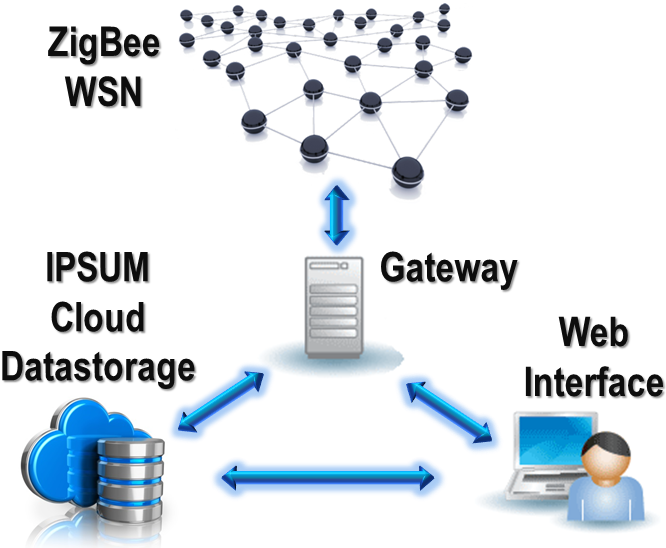
\includegraphics[width=0.48\textwidth]{thesis}
%\rule{30em}{0.5pt}
\caption{Presentation of the subject}
\label{fig:thesis}
\end{figure} 




%----------------------------------------------------------------------------------------

%-------------------------------------------------------------------
\subsection{API Frame Specifications}
To communicate with the ZigBee radio there are 2 modes, AT (transparent mode) and API (application programming interface). AT mode means that what you send to the zigbee radio using RS232, the ZigBee radio will send to its default destination. Unless you send “+++”, wait for the ZigBee to reply with OK, and then send an AT command. AT commands are used to change the configuration of the ZigBee radio. For instance the AT command OP requests the operating PAN ID.\\
AT mode is fairly limited and only good for point to point communication since you can’t really specify the destination unless you change the default destination all the time. So that is why the sensor network operates in API mode. This means that everything sent to the zigbee radio, using serial communication, is now packetized.\\
API defines a number of different packets as can be found in chapter 9 of \defcitealias{XBEE}{XBee/XBee-Pro ZB RF Modules User Manual, 2012}\citepalias{XBEE}. An API packet is shown in figure \ref{fig:api}. It starts with 0x7E as start delimiter and is followed by the length of the data excluding checksum. Then a API-specific structure follow which depends on the type of packet.\\
\begin{figure}[htbp]
\centering
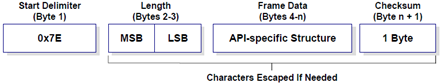
\includegraphics[width=0.48\textwidth]{api}
\caption{UART Data Frame Structure}
\label{fig:api}
\end{figure} 
\begin{table}[!ht]
\begin{center}
\begin{tabular}[!ht]{|c|c|}
\hline
\textbf{API Frame Name} & \textbf{API ID}\\
\hline
AT Command & 0x08\\
\hline
ZigBee Transmit Request & 0x10\\
\hline
AT Command Response & 0x88\\
\hline
ZigBee Receive Packet & 0x90\\
\hline
\end{tabular}
\caption{API Frame Names and Values}
\label{tab:apis}
\end{center}
\end{table}\\
\label{api1}\noindent
A reduced list of possible packets can be found in table \ref{tab:apis} (for the full list please see appendix \ref{AppendixF}). As mentioned an AT command is used to alter configurations of the ZigBee radio. This can of course also be done in API mode. For details about all the packets, please consult the datasheet. The only packets types used in this project are: 'ZigBee transmit request, 0x10' and 'Zigbee receive packet, 0x90'.\\
A ZigBee transmit request is shown in figure \ref{fig:api4}. This packet is used to send data from this ZigBee radio to a remote one. All that has to be known is the remote ZigBee address. These types of packets are constructed by the gateway to send out data to the libelium nodes but also by libelium nodes to send data to other libelium nodes or the gateway. Libelium has its own specific format for the RF Data as will be explained in section \ref{libPAQ}. To reach the gateway the address of the coordinator can be used, since the coordinator and gateway in our case are the same. This is convenient since the coordinator can always be addressed with 0x0000000000000000. The reason we chose the gateway and coordinator to be the same is that the coordinator receives a lot of traffic due to its role as coordinator and the same goes for the gateway. So these 2 devices should be in the center of the network for efficiency reasons. Assigning one device for these 2 roles and trying to position this device as central as possible will ask for the least amount of routing overhead.\\
When data is received by a ZigBee radio, this radio will send out a Zigbee receive packet via its serial communication. An example of this packet can be found in figure \ref{fig:api5}. Again the received data has an additional format as specified by Libelium.
\vfill 